In 1999, Banaszek et. al. made direct optical measurements on a number of optical quantum states. Their experimental set-up was fairly simple and the post-processing on their acquired data was relatively trivial. The set-up for their experiment is shown in figure \ref{BanaSetUp}. Typically, the method to determine the Wigner function for a quantum state is to, first, determine the density matrix representation of the state and, second, using the equivalence between the density matrix and the Wigner function, transform the data into the Wigner state-space representation. There are a number of reasons this is typically done. However, the inversion that is needed to go from the discrete density matrix representation to the continuous state-space representation is non-trivial. It typically involves heavy statistics (maximum likelihood estimation theorems to determine which state the data represents) and awkward filtered back-projection schemes analogous to those used in the medical field to render images of the human body using tomography machines (PET, CT, MRI, etc.). There is no utility to this process since the density matrix is the fundamental data set and has just as much information as the Wigner representation.

\begin{figure}%
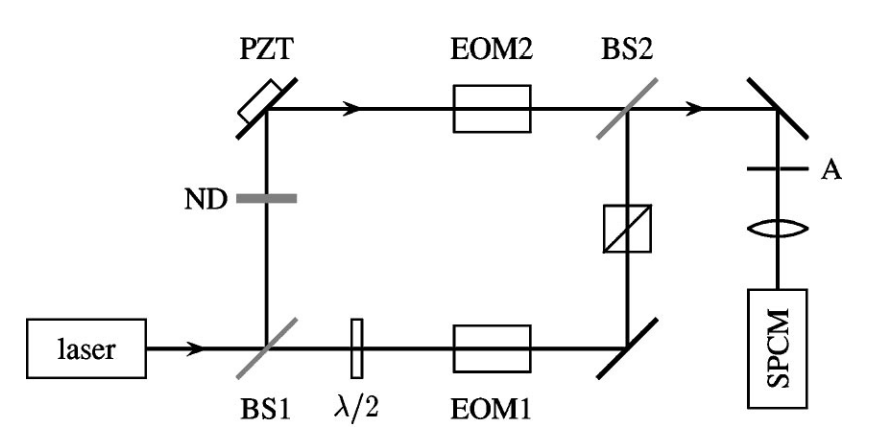
\includegraphics[width=300px,height=153px]{Figures/BanaSetUp.png}%
\caption{Set-up of the optical experiment conducted by Banaszek et. al. in 1999.}%
\label{BanaSetUp}%
\end{figure}

However, Banaszek et. al. implemented a direct measurement of the Wigner function of the quantum state of optical light. The key to sidestepping all the statistics is to realize that the Wigner representation of the state of light (expressed in terms of the displacement of the amplitude of light in phase space) is given by: $W(\alpha)=\frac{2}{\pi}Tr[D(-\alpha)\rho D(\alpha)e^{i\pi N}]$ \cite{Deleglise} which Banaszek et. al. express, equivalently, as  $W(\alpha)=\frac{2}{\pi}\sum_{n=0}^{\infty}(-1)^n D(\alpha)\ket{n}\bra{n} D^\dagger(\alpha)$. Thus, by sweeping $\alpha$ (the phase space parameter), and projecting the resulting quantum state onto the Fock basis, one can determine $W(\alpha)$. Physically, Banaszek et. al. implemented a sweep of $\alpha=|\alpha|e^{i\theta}$ through the use the two branches of their Mach-Zehnder interferometer: a half-wave plate, a Pockels cell (which is a tunable wave plate, called EOM2) and a polarizer control the magnitude of $\alpha=$, $|\alpha|$, while the upper branch, consisting of a neutral density filter (ND) and an electro-optic phase modulator (EOM2) controls the angle of $\alpha$, $\theta$, in phase space; see figure \ref{BanaSetUp}. The measurement of the light is done with a single photon counting module (SPCM). This projects the state of light onto the Fock basis. The piezoelectric translator (piezoelectric mirror, called PZT) is used only for one data set. For this data set, the translator is modulated with a high-frequncy drive, altering the phase of $\alpha$ over very short time scales. In a similar manner as Smithey et. al. \cite{Smithey}, Banaszek et. al. adjusted the amplitude and phase of $\alpha$ in discrete amounts: they used 20 amplitudes and 40 phases of $\alpha$. Many trials are conducted at a particular amplitude and phase, $\alpha_i$ to obtain a distribution over Fock states. Then, $W(\alpha_i)$ is determined. Then, the phase and/or amplitude is adjusted and another multitude of measurements is made. The results of their experiment are shown in figure \ref{BanaResults}.



\begin{figure}%
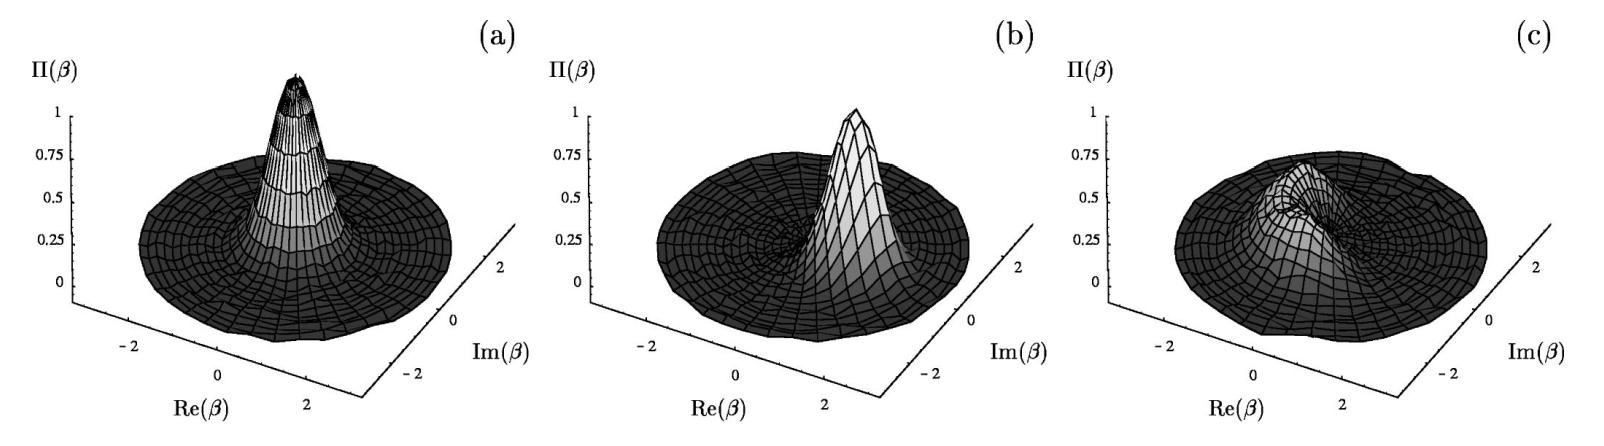
\includegraphics[width=400px,height=111px]{Figures/BanaResults.png}%
\caption{Measured results of three quantum states prepared by Banaszek et. al. Panel a) corresponds to measurements conducted on the vacuum state. Panel b) corresponds to measurements of a weakly displaced vacuum state. Panel c) corresponds to the coherent state whose phase was modulated using the piezoelectric mirror. $\beta=e^{i\theta}\sqrt{n_{vac}}$. Note that $\beta$ is simply a scaled version of $\alpha$.}%
\label{BanaResults}%
\end{figure}